%% ============================================================================
%% pnas_outline.tex — PNAS research-article TEMPLATE / OUTLINE (not a draft)
%% for the rank-diffusion paper. 2026-07-05.
%%
%% WHAT THIS FILE IS
%%   A compilable skeleton at section -> subsection -> paragraph granularity.
%%   Every planned paragraph carries a rendered PLAN block (job / topic+
%%   transition direction / numbers with MODEL_STATUS \S citations / claim
%%   flags). No article prose is drafted here. Empirical values appear ONLY
%%   inside PLAN blocks with their source section; anything unsourced is a
%%   \todo{}. Set \plansfalse below to hide all PLAN blocks while drafting.
%%
%% HOW TO COMPILE
%%   cd paper && pdflatex pnas_outline && pdflatex pnas_outline
%%   Uses the official PNAS class shipped in this directory (pnas-new.cls,
%%   pnasresearcharticle.sty, widetext.sty, pnas-new.bst). Figures 2-4 are
%%   included from ../figures/ (committed); Figures 1 and 5 are placeholder
%%   boxes because they DO NOT EXIST YET (specs in their captions).
%%   Verified compiling with pdflatex (TeX Live 2024); tectonic not installed.
%%
%% SOURCE DOCUMENTS (repo-relative; the outline cites them throughout)
%%   llm_fitting/MODEL_STATUS.md            — canonical record ("\S2x" = its section 2x)
%%   llm_fitting/reviews/gpt55_pro_review_2026-07-05.md          — review #1 (E2 abstract, E3 figures)
%%   llm_fitting/reviews/gpt55_pro_revised_verdict_2026-07-05.md — revised verdict (\S4 = approved claim sentences)
%%   llm_fitting/research_notes.md          — \S6c-6d positioning, \S7 sources
%%   llm_fitting/SI_DISCOVERY_CHRONOLOGY.md — discovery-vs-confirmation table (-> SI-7)
%%   llm_fitting/CONFIRMATION_PROTOCOL.md   — registered, NOT YET RUN (-> slots here)
%%   llm_fitting/make_figures.py            — generates Figs 2-4
%%
%% ----------------------------------------------------------------------------
%% CONTRADICTIONS / FLAGS FOUND WHILE ASSEMBLING THIS OUTLINE (not resolved
%% here; the research log is write-only for this task):
%%   1. The E2 draft abstract (review #1) PREDATES the binding claim set:
%%      it says "independently identified measurement noise" where \S2r/\S2x
%%      require "identified in shape everywhere, in level at the FB head,
%%      bounded in level elsewhere"; and "lifecycle-scale movement" where the
%%      binding language is "excess low-frequency structure". The abstract
%%      slot below flags both edits. E2 is kept verbatim as a comment.
%%   2. README rounds the b block-bootstrap CIs ([0.94,1.06] FB /
%%      [0.96,1.11] comments) vs \S2u's [0.939,1.064] / [0.958,1.108] —
%%      cosmetic, but the paper should quote \S2u.
%%   3. research_notes.md's trailing "Last updated: 2026-07-03" line predates
%%      its own 2026-07-05 positioning section — cosmetic.
%%   4. Review #1's Fig 3 plan says "before/after pin"; the built
%%      fig3_sigma_obs.png shows the superseded legacy floor as a dashed
%%      reference instead — the built version is the reconciled spec.
%%
%% ----------------------------------------------------------------------------
%% PNAS STATED PREFERENCES (checked 2026-07-05; pnas.org serves 403 to
%% non-browser fetchers, so triangulated from the NAS-maintained 2025
%% Overleaf template's embedded guidance + secondary summaries — all agree):
%%   - Research articles: 6 pages PREFERRED, including title/authors/
%%     abstract/Significance/main text/references/figure legends; "keep the
%%     text under 39,000 characters (including spaces)" ~= 4,000 words of
%%     body text with ~50 references and ~4 medium display items. Hard
%%     ceiling 12 pages, ~$375/typeset page beyond the limit. (The old
%%     "figures = 250-word equivalents" phrasing is legacy; the operative
%%     rule is character-displacement/page-based, same effect.)
%%   - Abstract: <= 250 words, single paragraph, no citations, "explain to
%%     the general reader the major contributions".
%%   - Significance statement: required, 50-120 words (system-enforced),
%%     "understandable to an undergraduate educated scientist outside their
%%     field of speciality".
%%   - Display items: no hard cap — they compete for the 6-page budget;
%%     stated norm ~4 medium items. Column width 8.7 cm; wide figures 11.4
%%     or 17.8 cm; panel labels uppercase italic A, B, C.
%%   - SI Appendix: single PDF, no length limit, max 10 SI files; "the main
%%     text must stand on its own without the SI"; if the paper is
%%     fundamentally about a new method, the method must be complete in the
%%     main text (RELEVANT HERE: the identification strategy is arguably the
%%     method contribution — its LOGIC stays in R2/R3, derivations to SI).
%%   - Section order (template's suggested): Abstract, Significance,
%%     Results, Discussion, Materials and Methods, Acknowledgments,
%%     References — "other orders and headings are permitted"; the intro is
%%     written WITHOUT a heading; Results subheadings are the norm.
%%   - References numbered by appearance, "(1, 2)" style, ~50 typical.
%%
%% REVEALED PREFERENCES — STRUCTURAL-MODEL SURVEY (10 verified post-2020
%% PNAS research articles; all checked against PNAS DOIs/PMC full text):
%%   1. Meng et al. 2025, "Spreading dynamics of information on online
%%      social networks", PNAS 122(4):e2410227122, 10.1073/pnas.2410227122.
%%      Structure: empirical fact subhead -> "Unified Equation" -> per-
%%      platform fits (WeChat/Weibo/Twitter, dataset table) -> universality/
%%      interpretation -> implications -> Conclusion+Discussion -> M&M;
%%      4 figs + 1 table; 17-section SI.
%%      Borrowed: THE ARC — cross-platform regularity, one concise equation
%%      with interpretable identified parameters, per-platform fits,
%%      universality section; and the main-text panels/datasets table.
%%   2. Sun, Caccioli & Livan 2023, "Ranking mobility and impact inequality
%%      in early academic careers", PNAS 120(34):e2305196120,
%%      10.1073/pnas.2305196120.
%%      Structure: descriptive rank-transition fact first, then a random-
%%      walk null to show rank stability exceeds baseline, then validation;
%%      exactly 4 figs + 1 table; analogy-driven Significance (Great Gatsby
%%      curve); 25 SI figures.
%%      Borrowed: the fact-then-null-adjudication sequencing (= our
%%      Eulerian stability vs persistence baseline), the display-item
%%      economy, and the Significance register.
%%   3. Li, Wang, Liu, Small & Gao 2022, "A spatiotemporal decay model of
%%      human mobility when facing large-scale crises", PNAS 119:
%%      e2203042119. One law collapses heterogeneous datasets, model then
%%      predicts held-out behavior; 5 figs; 71-figure SI.
%%      Borrowed: the data-collapse + out-of-sample-prediction figure
%%      grammar (our Figs 1 and 5); license for a heavy robustness SI.
%%   4. Kawakatsu, Chodrow, Eikmeier & Larremore 2021, "Emergence of
%%      hierarchy in networked endorsement dynamics", PNAS 118(16):
%%      e2015188118. Model-first; 4 figs + 2 tables; per-dataset parameter
%%      table compared against a theoretically meaningful threshold.
%%      Borrowed: the parameter-table convention — per-platform estimates
%%      vs the b=1 threshold (candidate second table, see Table 1 block).
%%   5. Chu & Evans 2021, "Slowed canonical progress in large fields of
%%      science", PNAS 118(41):e2021636118. Mechanism + numbered predictions
%%      up front, one figure per prediction; paradox-as-headline
%%      Significance.
%%      Borrowed: the paradox framing — churn underneath, frozen aggregate
%%      structure — rhetorically our exact fact.
%%   6. Hosseinmardi et al. 2021, "Examining the consumption of radical
%%      content on YouTube", PNAS 118(32):e2101967118. Methods BEFORE
%%      Results; 7 figs + 2 tables.
%%      Borrowed: proof that >6 display items and nonstandard order are
%%      tolerated when measurement is the contribution; the numbered
%%      findings-preview paragraph (our Intro par. 4).
%%   7. Hosseinmardi et al. 2024, "Causally estimating the effect of
%%      YouTube's recommender system using counterfactual bots", PNAS
%%      121(8):e2313377121. Results organized by experiments; ~6 figs + 2
%%      tables.
%%      Borrowed: foregrounding the baseline comparison (their bots = our
%%      persistence baseline) as the evidentiary spine of Results.
%%   8. Lera, Pentland & Sornette 2020, "Prediction and prevention of
%%      disproportionally dominant agents in complex networks", PNAS
%%      117(44):27090. Theory-first econophysics in 6 pages with only 2
%%      dense multi-panel figures.
%%      Borrowed: figure economy for the identification-region figure
%%      (our Fig 3's bounded-bracket shading); NOT its theory-first order.
%%   9. Ke, Gates & Barabási 2023, "A network-based normalized impact
%%      measure...", PNAS 120(48):e2309378120. Introduce quantity ->
%%      validate against ground truth -> then trust it for discovery;
%%      7 figs.
%%      Borrowed: the introduce-validate-use ladder for sigma_obs (R3:
%%      identify it, audit it, then rely on it in R5).
%%  10. Musso, Rybski, Helbing & Neffke 2026, "Large cities lose their
%%      growth advantage as countries urbanize", PNAS 123(26):e2529430123.
%%      Purpose-built consistently-defined datasets as a first-class
%%      contribution; revision-of-a-classic-scaling-law narrative.
%%      Borrowed: framing the era-disciplined panels + census/tracked
%%      distinction as a data contribution, not housekeeping (SI-1/SI-2
%%      get cited from the main text as assets).
%%   Dropped after verification: Allen et al. 2020 "fake news problem" is
%%   Science Advances, not PNAS; Iñiguez et al. 2022 "Dynamics of ranking"
%%   is Nature Communications (cited as literature, not as a structural
%%   model); Watts et al. 2021 news measurement is a PNAS perspective.
%%
%%   PRIMARY STRUCTURAL MODEL: Meng et al. 2025 (#1) — same paper-shape at
%%   the same journal; our Results subheads R1-R5 map one-to-one onto its
%%   sequence (fact -> equation -> identification/fits -> validation ->
%%   interpretation). CO-PRIMARY: Sun, Caccioli & Livan 2023 (#2) —
%%   nearest subject cousin; calibrates display-item economy (4-5 figs + 1
%%   table) and the Significance pitch. Li 2022 (#3) is the reference for
%%   Figs 1/5; Kawakatsu 2021 (#4) for the parameter-table option.
%%
%%   STATED-VS-REVEALED CONFLICTS OBSERVED (we side with revealed where
%%   they diverge): display items stated ~4, revealed 2-9 (we plan 5 figs +
%%   1 table); "main text stands alone" stated, revealed practice loads
%%   extreme robustness into SI (Li: 71 SI figures) — we do the same via
%%   SI-1..SI-10; section order flexible in practice (we keep the default);
%%   6 pages preferred but 12 permitted with page charges — if the two-
%%   estimand exposition needs it, 7-8 pages is an accepted cost, decided
%%   at drafting time, not by cutting the claim-discipline material.
%%
%% ----------------------------------------------------------------------------
%% THE THREE BIGGEST STRUCTURAL RISKS FOR ACCEPTANCE, AND HOW THIS OUTLINE
%% MITIGATES EACH (per the revised external verdict \S2 and \S7):
%%   RISK 1 — BREADTH (n=2 platforms; "universality" is the currency at PNAS).
%%     Mitigation: the DESCRIPTIVE FACT leads and is framed as the paper's
%%     citable object (Fig 1, R1); the model earns its keep via identification
%%     + prediction, not via universality claims; "law" language is scoped
%%     ("approximately factorized", "across Facebook tracked activity and
%%     Reddit census attention"); R6 + SI-9 give breadth results a natural
%%     slot WITHOUT the current spine depending on them.
%%   RISK 2 — CONFIRMATION PENDING (revised verdict A1: "do not submit to
%%     PNAS before the registered comments extension is run").
%%     Mitigation: marked result slots (R5 last paragraph + SI-8) support
%%     both sequencings — (a) hold submission until E1-E4 are run (verdict's
%%     recommendation, the default), or (b) submit as explicit model
%%     discovery with the frozen protocol disclosed. The slots are written
%%     so either fill is a one-paragraph edit, not a restructure.
%%   RISK 3 — SPECIFICATION-SEARCH APPEARANCE (structure stack vs movement
%%     stack; six months of sequential model changes).
%%     Mitigation: the two-estimand design is a MAIN-TEXT paragraph with its
%%     mechanism stated (long-horizon D(h) moments identify slow structure
%%     on full panels, destabilize short rolling train windows — \S2s), plus
%%     Table 1 with an explicit "target" column (verdict A4); SI-7 imports
%%     the dated discovery chronology; SI-8 shows the protocol was frozen
%%     before the extension was touched.
%% ============================================================================

\documentclass[9pt,twocolumn,twoside]{pnas-new}
% SWAP-IN NOTE: this compiles against the official pnas-new.cls in this
% directory. If the class ever goes missing, replace the two lines above/below
% with `\documentclass[twocolumn]{article}` plus stubs for \templatetype,
% \significancestatement, \matmethods, \showmatmethods, \acknow, \showacknow,
% \dropcap, \leadauthor, \authorcontributions, \authordeclaration,
% \correspondingauthor, \keywords, \dates — all PNAS-specific.
\templatetype{pnasresearcharticle}

\usepackage{graphicx}
\graphicspath{{../figures/}{figures/}}

%% ---- outline machinery (delete at drafting time) ---------------------------
\newif\ifplans\planstrue  % \plansfalse hides every PLAN block
\newcommand{\todo}[1]{\textcolor{red!65!black}{\textbf{[TODO: #1]}}}
% \PLAN{job}{topic-sentence direction + transition}{numbers w/ sources}{claim flags ('' if none)}
\newcommand{\PLAN}[4]{\ifplans\par\begingroup
  \footnotesize\sffamily\color{black!60}%
  \noindent\rule{\linewidth}{0.4pt}\par
  \textbf{JOB:} #1\par
  \textbf{DIRECTION:} #2\par
  \textbf{NUMBERS:} #3\par
  \if\relax\detokenize{#4}\relax\else\textbf{CLAIM FLAGS:} #4\par\fi
  \noindent\rule{\linewidth}{0.4pt}\par
\endgroup\fi}
% Word-count target tag, rendered after each \section
\newcommand{\WT}[1]{\ifplans{\par\noindent\footnotesize\sffamily\color{black!60}[section target: #1 words]\par}\fi}
%% ----------------------------------------------------------------------------

%% ============================================================================
%% WORD BUDGET (body text; targets sum to 4,000 = the stated ~39,000-char /
%% 6-page preference; NOTE the 6-page count also charges figure legends and
%% references against the pages, and we carry 6 display items vs the ~4-item
%% norm — so 6 pages is TIGHT and 7 pages is the realistic landing zone; the
%% 12-page ceiling with page charges is the accepted escape valve, per the
%% revealed-preference survey above):
%%   Introduction ................. 450
%%   R1  The fact ................. 550
%%   R2  The model ................ 400
%%   R3  Identification ........... 500
%%   R4  One amplitude ............ 350
%%   R5  Validation ............... 600
%%   Discussion ................... 500
%%   Materials and Methods ........ 650   (small type; details -> SI)
%%   TOTAL ........................ 4,000
%% Figure legends: budget ~120-150 words each (x6 display items), on top.
%% If 6 pages must bind: cut order is M&M 650->500 (push blocks 2/4 to SI),
%% Discussion 500->450, R1 550->500. If expanding to 7-8 pages: expand R5
%% (validation detail) and R3 first — they carry the referee load.
%% ============================================================================

%% ---- TITLE CANDIDATES (pick one; rationale one line each) -------------------
%% T1. "Eulerian stability with Lagrangian churn in digital attention
%%      rankings" — leads with the named descriptive fact (the citable,
%%      teachable object); the coinage is the paper's hook and the term the
%%      field would adopt. RECOMMENDED WORKING TITLE.
%% T2. "Digital attention rankings are stable in shape but unstable in
%%      membership" — declarative-sentence title (a common PNAS pattern);
%%      states the fact with zero jargon; loses the coinage.
%% T3. "A factorized rank-diffusion law for online attention" — model-first
%%      and shortest; risks burying the descriptive hook that referees and
%%      readers reward; "law" invites the n=2 breadth objection in the title.
%% T4. "Stable ranks, churning identities: a validated stochastic model of
%%      online attention hierarchies" — two-beat fact + model; "validated"
%%      signals the OOS contribution; slightly long.
%% T5. "One process, one amplitude: rank stability and identity churn across
%%      online attention platforms" — foregrounds the b=1 factorization
%%      (Q-model echo); best if breadth systems land before submission.
\title{Eulerian stability with Lagrangian churn in digital attention rankings}

%% PNAS first-page banner: article type / classification (placeholder —
%% likely dual classification: Social Sciences; Applied Physical Sciences).
%% NOTE: PNAS_Logo.pdf in this directory is a PLACEHOLDER (the official
%% logo ships with the journal's production files, not with the class).
\articletype{Social Sciences (classification placeholder)}

%% ---- authors/affiliations: placeholders -------------------------------------
\author[a,1]{Author One}
\author[b]{Author Two}
\affil[a]{Affiliation One, Department, University, City, Country}
\affil[b]{Affiliation Two}
\leadauthor{One}
\authorcontributions{Please provide details of author contributions here.}
\authordeclaration{The authors declare no competing interest.}
\correspondingauthor{\textsuperscript{1}To whom correspondence should be addressed. E-mail: author.one@example.edu}

%% ---- SIGNIFICANCE STATEMENT SLOT --------------------------------------------
%% Guidance (50-120 words, system-enforced; "an undergraduate educated
%% scientist outside their field"; no jargon, no citations; pitch register
%% modeled on Sun/Caccioli/Livan 2023's analogy-driven statement):
%%   Sentence 1-2: the descriptive fact FIRST, in plain words — online
%%     attention rankings keep the same shape year after year while the
%%     accounts occupying each rank continuously change; this pattern has not
%%     been documented before.
%%   Sentence 3: what we add — a compact stochastic model whose noise level is
%%     pinned down by independent measurements and which predicts NEXT
%%     season's rank movement, not just past patterns.
%%   Sentence 4: why it matters — the concentration of online attention is
%%     structural (the ladder persists) even though individual success is
%%     transient (occupants churn); relevant to platform power, creator
%%     economies, and information diversity debates.
%%   Claim flags: FB = "of tracked activity"; do not say "universal law".
\significancestatement{\todo{Significance statement per the guidance block in the source comments — descriptive fact first, model second, stakes third; $\le$120 words.}}

\keywords{attention dynamics $|$ ranking dynamics $|$ rank diffusion $|$ measurement error $|$ out-of-sample validation}

%% ---- ABSTRACT SLOT -----------------------------------------------------------
%% E2 DRAFT ABSTRACT (review #1, verbatim; STRONG PRIOR, NOT GOSPEL —
%% two edits are REQUIRED by the binding claim set before use):
%%   (i)  "independently identified measurement noise" -> scope per \S2r:
%%        identified in shape everywhere, in level at the FB head, bounded
%%        in level elsewhere (e.g. "measurement noise bounded by an
%%        independent daily-replication instrument").
%%   (ii) "lifecycle-scale movement" -> "excess low-frequency structure"
%%        (\S2v/\S2x binding language).
%%   Optionally add the conservative bound b in [0.94, 1.11] (\S2u).
%% ---- E2 verbatim:
%%   Digital attention rankings are stable in shape but unstable in
%%   membership: the same ranks persist while the pages, subreddits, and
%%   endpoints occupying them churn. We model this "Eulerian stability with
%%   Lagrangian churn" using a rank-conditional stochastic process with
%%   rebirth at the lower boundary, independently identified measurement
%%   noise, and one persistent entity-level amplitude. Across Facebook pages
%%   and Reddit subreddit attention, weekly log activity is well described by
%%   a slow rank-dependent home, short-run transitory movement, a stationary
%%   platform level, and lognormal endpoint temperament. A horizon-dispersion
%%   test shows that the same amplitude scales transitory and permanent
%%   movement to first order (b~1), with small super-unit deviations. The
%%   model reproduces rank-size stability, occupant turnover, and held-out
%%   displacement distributions, beating or matching persistence baselines in
%%   rolling-origin tests. The remaining discrepancies concentrate in
%%   measurement alignment and lifecycle-scale movement. The results suggest
%%   a parsimonious factorized law for the head of digital attention
%%   rankings.
\begin{abstract}
\todo{Abstract ($\le$250 words; target $\approx$150). Start from the E2 draft in the source comments and apply the two binding-claim-set edits flagged there.}
\end{abstract}

\dates{This manuscript was compiled on \today}

\begin{document}

\maketitle
\thispagestyle{firststyle}
\ifthenelse{\boolean{shortarticle}}{\ifthenelse{\boolean{singlecolumn}}{\abscontentformatted}{\abscontent}}{}

%% ============================================================================
%% INTRODUCTION (no heading in PNAS format; opens with dropcap)
%% ============================================================================
\WT{450}

\dropcap{I}\todo{Intro paragraph 1}
\PLAN{Hook: state the unpublished descriptive fact in one breath — attention
rankings hold their shape while their membership churns — and name it
(Eulerian stability with Lagrangian churn).}
{Open on the object everyone knows (leaderboards / most-engaged pages /
top subreddits), then the two-sided observation: photograph the ladder twice
a year apart and it looks identical; track who stands on each rung and almost
everything has moved. Hand to par.\ 2: why neither existing tradition
predicts this conjunction.}
{Teaser numbers, sourced: FB rank-1 changes hands 52\%/week (\S2m item 2);
19 distinct \#1 pages in 86 weeks (\S2o); rank-size overlay dispersion for
Fig 1A \todo{compute for Fig 1}.}
{FB language "of tracked activity" from the FIRST mention; this fact is
unpublished — claim novelty explicitly but verifiably ("has not, to our
knowledge, been documented").}

\todo{Intro paragraph 2}
\PLAN{Position against the two literatures that each explain half the fact.}
{Size-distribution / random-growth tradition (Gabaix 1999; Luttmer 2007;
Axtell 2001; Atlas models) explains stationary ladders but is silent on who
occupies the rungs; ranking-dynamics work (I\~niguez et al.\ 2022; Blumm et
al.\ 2012) documents churn regularities across many systems but with
qualitative model fits — no measurement-error model, no out-of-sample
prediction. Hand to par.\ 3: what an answer must therefore deliver.}
{No numbers; citations only (see bibliography plan).}
{Positioning is the differentiator list from research\_notes \S6c:
identification discipline, OOS validation, instrument forensics — state as
requirements here, claim them in par.\ 3.}

\todo{Intro paragraph 3}
\PLAN{State the answer: the approximately factorized rank-diffusion law
(the binding spine sentence).}
{The spine, adapted from MODEL\_STATUS \S6 addendum 2026-07-05 (binding):
a shared rank-conditional stochastic process with independently bounded
measurement noise and boundary rebirth, multiplied to first order by one
persistent endpoint amplitude — predicting held-out rank movement and
reproducing the main churn structure. Hand to par.\ 4: the evidence base and
its discipline.}
{b conservative bound $[0.94, 1.11]$, all central estimates $[0.98, 1.08]$
(\S2u); "to first order one persistent endpoint amplitude" (\S2x).}
{BINDING: "dominant one-amplitude factorization", NEVER "all heterogeneity
is amplitude" ($\kappa_i$ log-SD $\approx$ 0.30 measured, second-order,
\S2v); $\sigma_{\mathrm{obs}}$: identified in shape everywhere, in level at
the FB head, bounded elsewhere (\S2r).}

\todo{Intro paragraph 4}
\PLAN{Preview the evidence and its design discipline; set expectations for
the two-estimand structure.}
{Two platforms, three metric-eras (FB tracked interactions, Reddit
submission karma, Reddit comment karma); a censored instrument handled by
era segmentation; structure and movement evaluated by different stacks BY
DESIGN with the scope condition stated (long-horizon moments identify slow
structure on full panels, destabilize short rolling train windows). Close
the intro by flagging the registered confirmation protocol (and, if run by
submission, its outcome). Hands to R1.}
{Panels: FB Era A T=86, $\sim$14.4k pages/wk (\S2g); Reddit subs T=30
K=5{,}000 $\approx$ 89.2\% of weekly karma (\S2b); comments T=136
K=12{,}500 $\approx$ 98.8\% (\S2g P0).}
{Reddit = platform census (Pushshift); FB = tracked panel, NEVER
platform-census language (\S2g owner directive); the structure-vs-movement
distinction is MAIN TEXT, not SI (revised verdict A4).}

%% ============================================================================
\section*{Results}
%% ============================================================================

\subsection*{Stable ranks, churning occupants}
\WT{550}
%% ---- R1: the descriptive fact (Fig 1) --------------------------------------

\todo{R1 paragraph 1}
\PLAN{Introduce the data and the estimand population in two sentences each.}
{Name the three panels and the top-coverage universe rule (pre-registered
coverage K, absence-penalized permanent-rank membership, closed universe
with buffer); point to M\&M and SI-2. Hand to par.\ 2: with the population
fixed, the Eulerian half of the fact.}
{FB Era A: 86 complete weeks, $\sim$14{,}362 pages/wk median, enrollment
frozen (\S2g P0); top-3{,}500 = 89.7\% of tracked activity (\S2g P0).
Reddit subs: K=5{,}000 = 89.2\% of weekly karma, census (\S2b). Comments:
K=12{,}500, B=50k, $\approx$98.8\%, T=136, census (\S2g P0).}
{Coverage percentages are never compared across platforms as commensurable
(census vs tracked, \S2g); "of tracked activity" attached to every FB
share.}

\todo{R1 paragraph 2}
\PLAN{Establish Eulerian stability: the rank-size curve and per-rank shares
are nearly stationary.}
{Describe Fig 1A-B: weekly rank-size curves overlaid across the whole panel
collapse onto one curve; per-rank activity shares stationary over years.
Quantify the collapse. Hand to par.\ 3: the same weeks, viewed by identity.}
{\todo{dispersion statistic for the rank-size overlay (Fig 1 build)};
top-2 log-gap quarterly means 0.215/0.228/0.253/0.174 — stationary across
Era A (\S2o); platform level mean-reverts: level VR13 = 0.121 on comments
(\S2j).}
{}

\todo{R1 paragraph 3}
\PLAN{Establish Lagrangian churn: identities flow through fixed ranks
continuously.}
{Describe Fig 1C-D: rank-1 occupancy timeline; fixed-rank occupant turnover
at horizons 1/4/13 weeks; boundary out-flux and 4-week return. The churn is
not tail noise — it reaches rank 1. Hand to par.\ 4: the conjunction is the
puzzle.}
{FB rank 1 changes hands 52\%/wk (\S2m); 19 distinct \#1 pages / 86 wks,
occupancy-weighted amplitude BELOW population median (0.47 vs 0.71, \S2o);
$\sim$10\%/wk of top-K crosses the boundary, 33--38\% back within 4 wks
(research\_notes \S3); comments outfluxK 0.089--0.090 (\S2g-X P5).}
{}

\todo{R1 paragraph 4}
\PLAN{Sharpen the puzzle into model requirements.}
{Neither frozen hierarchy nor turbulent mixing: the conjunction demands a
process that holds the ladder invariant while moving its occupants — state
the three requirements a model must meet ((i) stationary ladder,
(ii) fixed-rank occupant turnover, (iii) held-out individual displacement;
\S6 framing). Hands to R2, which supplies the process.}
{No new numbers.}
{The requirements sentence is the paper's internal contract: R5 validates
exactly (i)--(iii), in that order.}

\subsection*{An approximately factorized rank-diffusion law}
\WT{400}
%% ---- R2: the model ----------------------------------------------------------

\todo{R2 paragraph 1}
\PLAN{Present the law compactly: one displayed equation plus a component
list in words.}
{Display the observation equation (revised verdict B2 form):
$X_{it}=\mu_{it}+\sqrt{v_i}\,\eta_{it}(z_i)+\lambda(z_i)L_t+\epsilon_{it}$
— slow OU home + fast (and, where identified, medium) transitory inside
$\eta$; lognormal amplitude $v_i$; stationary platform level $L_t$;
measurement noise $\epsilon$; Gabaix rebirth at the boundary of the
top-coverage universe. Rank-dependence enters through permanent-rank bands.
Hand to par.\ 2: every symbol has its own identifying moment.}
{Component parameters quoted later where used; here only the structure.
Amplitude spread $s$: FB 0.890, subs 0.941, comments 0.692 — metric-
dependent (\S2h); $\rho_L$ measured per platform: 0.48 FB / 0.90 subs /
0.82 comments (\S2j).}
{b=1 is the MAIN model; measured b is the refinement table (\S2x).
"Approximately factorized"; never "universal".}

\todo{R2 paragraph 2}
\PLAN{Give the identification map: which moment or instrument pins which
component — the paper's central methodological claim.}
{One sentence per pairing: home reversion $\kappa(z)$ from multi-horizon
change variances $D(h)$ (R3, Fig 2); $\sigma_{\mathrm{obs}}$ from two
independent instruments — weekly covariance structure and a daily-
replication noise floor (R3, Fig 3); amplitude spread $s$ from
bias-corrected log change-variance dispersion; the factorization exponent
$b$ from the horizon-dispersion moment $s(h)$ (R4, Fig 4); $\rho_L$ from
the platform-level path. Hand to par.\ 3: what is claimed and what is not.}
{Moment-to-parameter pairings as listed in \S2m ("every parameter is
identified from a declared moment or an independent instrument") — with the
\S2q E5 amendment: "or train-only-calibrated and declared".}
{Do NOT write "nothing is tuned" unqualified — the OOS gate's
$\sigma_{\mathrm{obs}}$ scale on the calibrated reference spec is
train-calibrated and must be called calibration (\S2q).}

\todo{R2 paragraph 3}
\PLAN{Claim discipline paragraph: state the law's scope before validating
it.}
{To first order, endpoint heterogeneity collapses to one amplitude
(the verdict-\S4.1 sentence, binding); residual reversion-rate
heterogeneity is measurable but second-order under the validation gates;
deviations are localized to excess low-frequency structure. Hands to R3.}
{$\kappa_i$ heterogeneity: conditioned split-half Spearman 0.346,
noise-corrected true log-SD 0.302 (\S2v).}
{BINDING sentence from revised verdict \S4.1; "excess low-frequency
structure" NEVER "lifecycle arcs" as lead language (\S2v/\S2x); arcs may be
named as one plausible source.}

\subsection*{Identification, not curve fitting}
\WT{500}
%% ---- R3: identification (Figs 2 and 3) --------------------------------------

\todo{R3 paragraph 1}
\PLAN{Show that slow reversion is invisible to short-lag autocovariances and
identified by long-horizon variance moments (Fig 2).}
{The change-autocovariance tail is flat in the home-reversion rate (the
classic mixture-of-exponentials degeneracy); appending $D(h)$ for
$h\in\{2,4,8,13,26,52\}$ makes the objective sharply V-shaped — the
Poterba--Summers/Cochrane long-horizon logic imported to attention panels.
Hand to par.\ 2: the noise level needs an instrument, not a moment.}
{SSE(a) flat under $\gamma_{0..6}$ (3e-6 to 1e-5 across the whole
$\kappa$ grid at a comments head knot); V-shaped with D(h); $\kappa$
interior 0.02--0.04 head/mid on comments (\S2i); scope condition: D(h)
moments destabilize SHORT rolling train windows — FB gate regression
0.114 to 0.179 (\S2i, \S2s).}
{The scope condition stated here is load-bearing for Table 1's two-stack
design — same mechanism, stated once, referenced there.}

\todo{R3 paragraph 2}
\PLAN{Measurement noise from two independent instruments; the bracket
language (Fig 3).}
{Spec-A: $\sigma_{\mathrm{obs}}$ from the weekly covariance structure.
Spec-B: a floor from daily-within-week replication, mapped through the
week-mean centering projection (the algebraically invariant "centered
floor"). Where they meet, the level is identified; elsewhere the truth is
bracketed. Hand to par.\ 3: the audit story that makes this credible.}
{FB head: Spec-A 0.176 vs centered floor 0.157 — agreement within
$\sim$12\%, level IDENTIFIED (\S2r). Subs head: 0.117 vs 0.074; comments
head: 0.120 vs 0.071 — bracketed (\S2r). Divergence grows with rank depth
on both platforms (posting intermittency question, \S2h).}
{BINDING: "identified in shape everywhere, identified in level at the FB
head, bounded in level elsewhere" (\S2r/\S2x). The cross-platform irony
(the platform WITHOUT daily history is the one with head identification) is
reportable (\S2r).}

\todo{R3 paragraph 3}
\PLAN{The centered-floor audit as an honesty exhibit (one short paragraph;
details SI-4).}
{An external audit found the original floor convention algebraically
unidentified (a null direction of the centering projection); adopting the
invariant centered floor both fixed the algebra and removed an internal
contradiction (the legacy floor sat ABOVE Spec-A on FB). All qualitative
conclusions survived the re-pin. Hands to R4.}
{Legacy-to-centered head shifts: subs 0.100 to 0.074 ($-26\%$), FB 0.207 to
0.157 ($-24\%$), comments 0.101 to 0.071 ($-30\%$) (\S2r); FB identified
gate result IMPROVED under the honest pin (0.211 to 0.152 uncond; 0.164 to
0.118 conditional) (\S2r).}
{Frame as discipline, not drama; the full algebra is SI-4.}

\subsection*{One amplitude per endpoint}
\WT{350}
%% ---- R4: the b=1 factorization (Fig 4) --------------------------------------

\todo{R4 paragraph 1}
\PLAN{Establish persistent entity-level amplitude heterogeneity and its
lognormal collapse (Fig 4A).}
{Per-entity change-variance dispersion is far beyond sampling noise and is
a persistent trait; corrected log change-variance distributions collapse
onto one lognormal across metrics; volatility belongs to the entity, not
the rank (fine-bands rejection, one sentence, details SI). Hand to par.\ 2:
does one amplitude scale everything?}
{Dispersion 15$\times$ (Reddit) / 35$\times$ (FB) pure $\chi^2$ noise;
split-half $\rho\approx0.6$ (\S2c); $s$ = 0.890 / 0.941 / 0.692 (FB / subs /
comments — metric-dependent, \S2h); fine-bands battery: variogram flat at
$\Delta r$=1, movers keep their own variance, shrunken history beats exact
rank (\S2c).}
{$s$ is metric- and universe-scale-dependent — do NOT write "one global
$s\approx0.9$" (\S2h "what broke" item 2).}

\todo{R4 paragraph 2}
\PLAN{The factorization test: s(h) flat implies one amplitude scales
permanent and transitory movement alike; b=1 not rejected time-aware
(Fig 4B-C).}
{The horizon-dispersion instrument $b=s(h^*)/s(1)$; entity bootstrap
rejects exact b=1, but block-bootstrap time-window uncertainty does not —
the excess is horizon-specific and carries the lifecycle-drift signature
(detrending moves comments toward 1). State the conservative bound; name
the Q-model analogy (one person-specific multiplier on a shared random-
impact rule). Hands to R5.}
{Point estimates b = 1.024 FB / 1.079 comments (\S2n); block-bootstrap 95\%
CIs [0.939, 1.064] / [0.958, 1.108]; detrended comments 1.059; common-
horizon h=4: 1.011 / 1.002; second-half comments 0.994; conservative bound
$b\in[0.94, 1.11]$ (\S2u).}
{b=1 is the MAIN model; measured b = refinement (verdict R4/B2, \S2x);
entity-vs-block bootstrap adjudication belongs in SI (verdict B2).}

\subsection*{Validation: descriptive cards, localized residuals, and
out-of-sample movement}
\WT{600}
%% ---- R5: validation (Fig 5 + Table 1) ---------------------------------------

\todo{R5 paragraph 1}
\PLAN{State the two-estimand design and its mechanism (Table 1).}
{Structure (in-sample moment reproduction) and movement (frozen rolling-
origin OOS displacement) are evaluated by different stacks BY DESIGN, with
the mechanism from R3 par.\ 1: long-horizon moments identify slow structure
on full panels and destabilize short train windows — demonstrated, not
asserted (the full stack was run through the gate and loses). Hand to
par.\ 2: the structure results.}
{FB full stack through the OOS gate: 0.170 $\pm$ 0.040 vs persistence
0.145 $\pm$ 0.031, coverage 20\% — LOSES, as the scope condition predicts
(\S2s).}
{This is Table 1's "target" column made prose (verdict A4); the failed run
is REPORTED — it is the anti-forking-paths exhibit (\S2s).}

\todo{R5 paragraph 2}
\PLAN{Descriptive structure cards with uncertainty; Q as residual
localization, never pass/fail.}
{FB Era A reproduces all 15 card moments at 20 simulation reps; subs 14/15;
comments 12/15. Covariance-weighted omnibus distances reject exact equality
— as expected at census-scale precision — and are used to LOCALIZE: every
dynamics block sits at Q/df 1--4 except the comments mid-horizon VR block
and the boundary-flux pair. Hand to par.\ 3: the harder test is held-out
movement.}
{FB 15/15, churn err 0.017--0.018, survives 20 reps (\S2p, \S2t); subs
14/15; comments 12/15 (\S2s); omnibus Q: FB 298, subs 217, comments 1275
vs $\chi^2$ df=15 reference $\approx$15--24 (\S2t); per-block Q/df table
(\S2y): FB VR 3.2 / ACF 3.5 / R2 0.7; comments VR 263.5, boundary 927.}
{BINDING: "15/15" is a descriptive scorecard; Q rejects exact equality and
localizes (\S2x; verdict \S4.3 sentence). Never "statistically
indistinguishable from data".}

\todo{R5 paragraph 3}
\PLAN{The movement gates: identified spec first, calibrated reference
parenthetical (Fig 5).}
{On FB Era A the identified Spec-B + conditional-state specification beats
persistence on 4/5 rolling splits with NO $\sigma_{\mathrm{obs}}$
calibration freedom, matching the calibrated benchmark in mean error (the
calibrated Spec-A stack beats 5/5 and is the parenthetical/SI reference).
Reddit submissions: conditional state beats 4/5. Comments — longest panel,
regime change inside it — at par with persistence with full bootstrap
median coverage. Hand to par.\ 4: what remains unexplained.}
{FB identified: 0.118 $\pm$ 0.038 vs 0.145 $\pm$ 0.031, cov 60\%, scale
1.0$\times$5 (\S2r); FB calibrated reference: 0.114 $\pm$ 0.046 vs 0.144
$\pm$ 0.030, 5/5, cov 60\% (\S2g-X P1); subs conditional: 0.118 $\pm$
0.061 vs 0.168 $\pm$ 0.004, 4/5, cov 100\% (\S2f); comments: 0.159 $\pm$
0.070 vs 0.160 $\pm$ 0.068, cov 100\%, last-split held-out distribution
exact at all horizons (\S2l).}
{BINDING ordering: identified Spec-B leads; calibrated 5/5 is
parenthetical/SI (verdict \S4.2, \S2x). Use the verdict's \S4.4 comments
sentence; never "comments passes".}

\todo{R5 paragraph 4}
\PLAN{Residuals: decomposed, bounded, and localized — not mysterious.}
{The one order-of-magnitude residual (comments mid-horizon VR block) is
decomposed by spectrum-preserving surrogates: roughly half is the scored-VR
functional's sensitivity to non-Gaussian phase/marginal structure (the
model's t-tails supply only $\sim$24\% of the data's discount), the rest a
genuine second-order mismatch of similar size; the demeaning signature is
"excess low-frequency structure", consistent with lifecycle arcs but not
uniquely so. Reversion-rate heterogeneity is real but bounded. Hand to
par.\ 5: the registered confirmation.}
{VR13 gap +0.078: $\approx$+0.03 non-Gaussian phase/marginal +
$\approx$+0.03--0.04 spectrum (\S2y); surrogate band vs data (\S2v);
$\kappa_i$ true log-SD 0.302 (\S2v); missingness explanation measured DEAD
(census 99.0\% present; censoring moves VR rows $<$0.001) (\S2w).}
{"Excess low-frequency structure" language (\S2x binding); the dead
missingness explanation is an SI negative result (verdict R6).}

\todo{R5 paragraph 5 — CONFIRMATION RESULTS SLOT}
\PLAN{Report the registered confirmation (or, if submitting pre-run,
disclose the frozen protocol as the design).}
{SEQUENCING A (default; verdict A1: do not submit before this is run):
one paragraph reporting E1 parameter transport (s, b, $\kappa(z)$ shape,
centered floor curve vs registered tolerances), E2 frozen-parameter
movement gate on the untouched 2021-07..2022-12 extension, E3 descriptive
card, E4 $\kappa_i$ concentration diagnostic — pass or fail, reported as
confirmation evidence either way. SEQUENCING B (explicit model-discovery
framing): state that the protocol is registered and frozen, cite SI-8, and
scope every law claim to the discovery panels. Hands to Discussion.}
{Registered pass criteria (CONFIRMATION\_PROTOCOL \S4): E1 s $\in$ [0.64,
0.74], b $\in$ [0.95, 1.15], floor within $\pm$25\% of 0.071 head to 0.248
deep; E2 rel err $\le$ persistence + 0.05 AND coverage $\ge$ 60\%; E4
predictive iff Spearman $\ge$ 0.20 AND concentration $\ge$ 1.3. Results:
\todo{E1}, \todo{E2}, \todo{E3 vs surrogate-adjusted target}, \todo{E4}.}
{Failures are findings about the law's domain, not prompts to refit
(protocol \S4); no post-hoc amendment.}

\todo{R5 paragraph 6 — OPTIONAL BREADTH SLOT (cut cleanly if unfilled)}
\PLAN{Breadth results, if available by submission: additional ranked
systems through the unchanged pipeline.}
{Claim to test on each new system: amplitude collapse (s(h) flat,
b $\approx$ 1) + OOS at-or-above persistence — NOT 15/15 everywhere
(\S2x agenda item 2). Wikipedia pageviews first (different institutional
measurement regime, clean daily data for Spec-B). One results sentence per
system; full cards to SI-9.}
{\todo{per-system s, b, OOS vs persistence, boundary flux}.}
{The current spine must not depend on this paragraph; it strengthens
"law" language but its absence changes no other claim.}

%% ============================================================================
\section*{Discussion}
\WT{500}
%% ============================================================================

\todo{Discussion paragraph 1}
\PLAN{Restate what was found at full altitude: the fact, the law, the
validation standard.}
{The conjunction (stationary ladder, churning occupants) is general across
two platforms and three metric-eras; a compact factorized process
reproduces it and predicts held-out movement; the validation standard
(identified/bounded measurement model, frozen OOS gates vs persistence,
instrument forensics, registered confirmation) is itself a contribution to
a literature that mostly reproduces stylized facts in-sample. Hand to
par.\ 2: interpretation.}
{One-sentence recap numbers only if needed: FB 4/5 identified OOS,
b $\in$ [0.94, 1.11].}
{Differentiators vs I\~niguez et al./Blumm et al. stated plainly but
respectfully (research\_notes \S6c strengths list).}

\todo{Discussion paragraph 2}
\PLAN{Interpret the factorization: what b=1 means for how attention
hierarchies work.}
{Positions are structural, occupants are exchangeable up to one persistent
amplitude — the attention analogue of the Q-model's person-specific
multiplier on a shared random-impact rule; connects the random-growth
tradition (ladder shape) to identity dynamics (who is on it). Implication:
durable concentration without durable incumbents; success at the head is
real (amplitudes persist) but tenure is stochastic. Hand to par.\ 3:
limits.}
{Rank-1 occupants are QUIETER than typical (occupancy-weighted
$\hat v$ = 0.47 vs median 0.71, \S2o) — the head churns because gaps are
tiny, not because occupants are loud.}
{Do not over-read: "to first order"; $\kappa_i$ axis exists (\S2v).}

\todo{Discussion paragraph 3}
\PLAN{Limitations, stated where a referee looks for them.}
{(i) Two platforms / three metrics: a shared model class with strong
internal validation, not yet a universal law — breadth is the test and the
pipeline is unchanged by design. (ii) FB is a censored tracked panel with
instrument eras; all FB claims are of tracked activity; era discipline in
SI-1. (iii) Confirmation status per the R5 slot. (iv) Residuals: excess
low-frequency structure and bounded reversion heterogeneity; the
$\sigma_{\mathrm{obs}}$ level below the head is bracketed, not identified.
Hand to par.\ 4: outlook.}
{$s$ varies by metric (0.69--0.94, \S2h) — the amplitude DISTRIBUTION is
metric-dependent even though the factorization is shared.}
{This paragraph is where the two review rounds' negotiated language pays
off — use it verbatim where possible (verdict \S4).}

\todo{Discussion paragraph 4}
\PLAN{Outlook and stakes.}
{What the law enables: forecasting movement distributions for real cohorts;
separating measurement regime from process when comparing platforms;
a quantitative baseline for interventions (algorithm changes, shocks)
against a null of factorized rank diffusion. Close on the attention-economy
stake: the stability of the attention hierarchy is a property of the
process, not of the incumbents.}
{No new numbers.}
{Keep speculation clearly marked; one paragraph only.}

%% ============================================================================
%% MATERIALS AND METHODS (rendered small, after Discussion, per PNAS format;
%% every subsection points to its SI section for the full treatment)
%% ============================================================================
\matmethods{%
\WT{650}

\todo{M\&M block 1 — Data and panels}
\PLAN{Sources, spans, and instrument status for each panel.}
{FB: CrowdTangle tracked-page panel, Era A 2020-11-02..2022-06-27 (86
complete weeks, $\sim$14.4k pages/wk, enrollment frozen); era segmentation
from collection metadata only, eras B/M excluded, C/D replication-only
(SI-1). Reddit: Pushshift census; submissions T=30; comments
2018-12..2021-06, T=136; day-count guard 0 flagged days (census property).
Instagram: query-censored negative control, never calibrated to (SI-9).}
{Era table + guard (\S2g P0); low-count-day guard: 60\% of trailing
28-day median, 59 flagged days, Spec-B drops flagged weeks, weekly fits
keep them (\S2g P0).}
{FB "of tracked activity"; absence is not behavior outside Era A (\S2g
directive 4).}

\todo{M\&M block 2 — Top-coverage universe and membership}
\PLAN{The estimand population.}
{Pre-registered coverage K from concentration statistics alone; closed
Lagrangian universe of B=4K entities by absence-penalized permanent rank;
weekly ranks recomputed within the universe; boundary flux is a tested
prediction, not an assumption. Membership-window drift measured and
headline-invariant (SI-2).}
{K values (\S2b, \S2g P0); membership overlap full vs half-window 0.73--
0.92, metrics move $<$ noise (\S2g-X P5); ghost-spiker pitfall and its
test (\S2b corrected pitfall).}
{}

\todo{M\&M block 3 — Estimators}
\PLAN{The moment/instrument stack, one sentence each.}
{Minimum-distance fit of change autocovariances $\gamma_{0..6}$ plus
multi-horizon variances D(h) per permanent-rank knot (OU home + AR fast
[+ AR medium] + noise); temperament s by limma-style digamma--trigamma
moment decomposition with Satterthwaite effective df; mix exponent
b = s(h*)/s(1); Spec-B centered daily-noise floor through the week-mean
centering projection; stationary level $\rho_L$ from the detrended
cumulative common-factor path. Weighting robustness: identity vs
precision-diagonal MD weighting is inert (SI-3).}
{$t$-tails df from within-entity excess kurtosis: 4.3 FB / 6.7 subs /
4.6 comments (\S2h); weighting audit: $\kappa$ grid-identical at 55$\times$
SE spread (\S2y).}
{"Identified from a declared moment or independent instrument, or
train-only-calibrated and declared" (\S2q E5).}

\todo{M\&M block 4 — Simulator and stacks}
\PLAN{Generative simulation and the two paper-primary stacks per panel.}
{MC simulation with entry/exit and rebirth; structure-primary stacks (full/
long) vs movement-primary stacks (short-window-safe), frozen per \S2s;
conditional forecasting = filtered end-of-train states (train-only
inputs).}
{Stack matrix (\S2s paper-primary declarations); conditional machinery
(\S2f; research\_notes \S6b).}
{}

\todo{M\&M block 5 — Scorecard, bands, and the OOS gate}
\PLAN{Evaluation machinery.}
{15-moment descriptive card; empirical bands by joint entity bootstrap +
moving-block week bootstrap; MC bands at 20 reps; omnibus Q with 50\%
diagonal shrinkage, decomposed by block; rolling-origin distributional OOS
gate ($\ge$5 splits, train-only estimation, persistence baseline,
bootstrap-CI coverage, Wasserstein), MOM\_FLOOR = 0.02 denominator rule.}
{Card definitions + Q construction (\S2t); gate protocol (\S2 and \S2q C4
fix); five splits are dependent — reported per-split (\S2q noted).}
{Q is a localization device (\S2x binding).}

\todo{M\&M block 6 — Code, data, and registration}
\PLAN{Availability + the frozen confirmation protocol pointer.}
{Code commit for the frozen evaluation (682d03f per CONFIRMATION\_PROTOCOL
\S1); registered protocol committed before any extension data was read;
data availability per platform (Pushshift public dumps; CrowdTangle
availability statement \todo{legal/ToS language for FB data sharing}).}
{Protocol registration date 2026-07-05, amendment A1 same day pre-data
(CONFIRMATION\_PROTOCOL \S6).}
{}
}%
\showmatmethods{}

\acknow{\todo{Acknowledgments — funding, data providers (Pushshift,
CrowdTangle), reviewers to thank.}}
\showacknow{}

%% Data availability statement (PNAS requires one):
%% \dataavail{...} — draft alongside M&M block 6; Pushshift dumps are public;
%% CrowdTangle terms need checking before promising raw-data release; code +
%% derived moment tables releasable.

%% ============================================================================
%% MAIN FIGURES — captions are SPECS (what each panel shows, axes, what the
%% reader must conclude), not final captions. Build status per figure.
%% ============================================================================

\begin{figure*}[p]
\centering
\fbox{\parbox[c][8cm][c]{0.94\textwidth}{\centering\sffamily
FIG 1 — DOES NOT EXIST YET. The paper's hook; build first.\\
Spec below; generator to be added to \texttt{llm\_fitting/make\_figures.py}.}}
\caption{\textbf{Fig.~1 spec — Eulerian stability with Lagrangian churn
(THE HOOK; most careful build).}
(\emph{A}) Rank-size overlay: weekly rank--activity-share curves for all
weeks of each panel (FB Era A, 86 weeks; Reddit comments, 136 weeks),
log-log, one translucent line per week atop the era median — reader
concludes the LADDER IS ONE CURVE (quantify overlay dispersion in an
inset; \todo{statistic}). Common-factor de-meaning noted in caption.
(\emph{B}) Per-rank share stationarity: activity share of fixed rank bands
(1--10, 11--100, 101--1000, 1001--K) as time series over the panel — flat
lines, reader concludes shares at each rung are stationary.
(\emph{C}) Occupant churn at fixed ranks: fraction of week-$t$ rank-band
occupants still in the band at $t+h$ for $h$ = 1, 4, 13, per band; plus the
rank-1 occupancy timeline (19 distinct \#1 pages / 86 wks on FB, \S2o;
rank 1 changes hands 52\%/wk, \S2m) — reader concludes IDENTITIES FLOW
THROUGH FIXED RANKS, all the way to rank 1.
(\emph{D}) Boundary exchange: weekly out-flux across rank K and 4-week
return rate (out $\sim$10\%/wk, return 33--38\%, research\_notes \S3) —
reader concludes the universe boundary is permeable and reflecting, not
absorbing. Panels A+B are the Eulerian half, C+D the Lagrangian half; the
caption's last sentence states the conjunction as the puzzle the paper
answers. Data: existing diagnostics already compute C--D quantities
(scorecard rows); A--B need a small new script.}
\label{fig:fact}
\end{figure*}

\begin{figure*}[p]
\centering
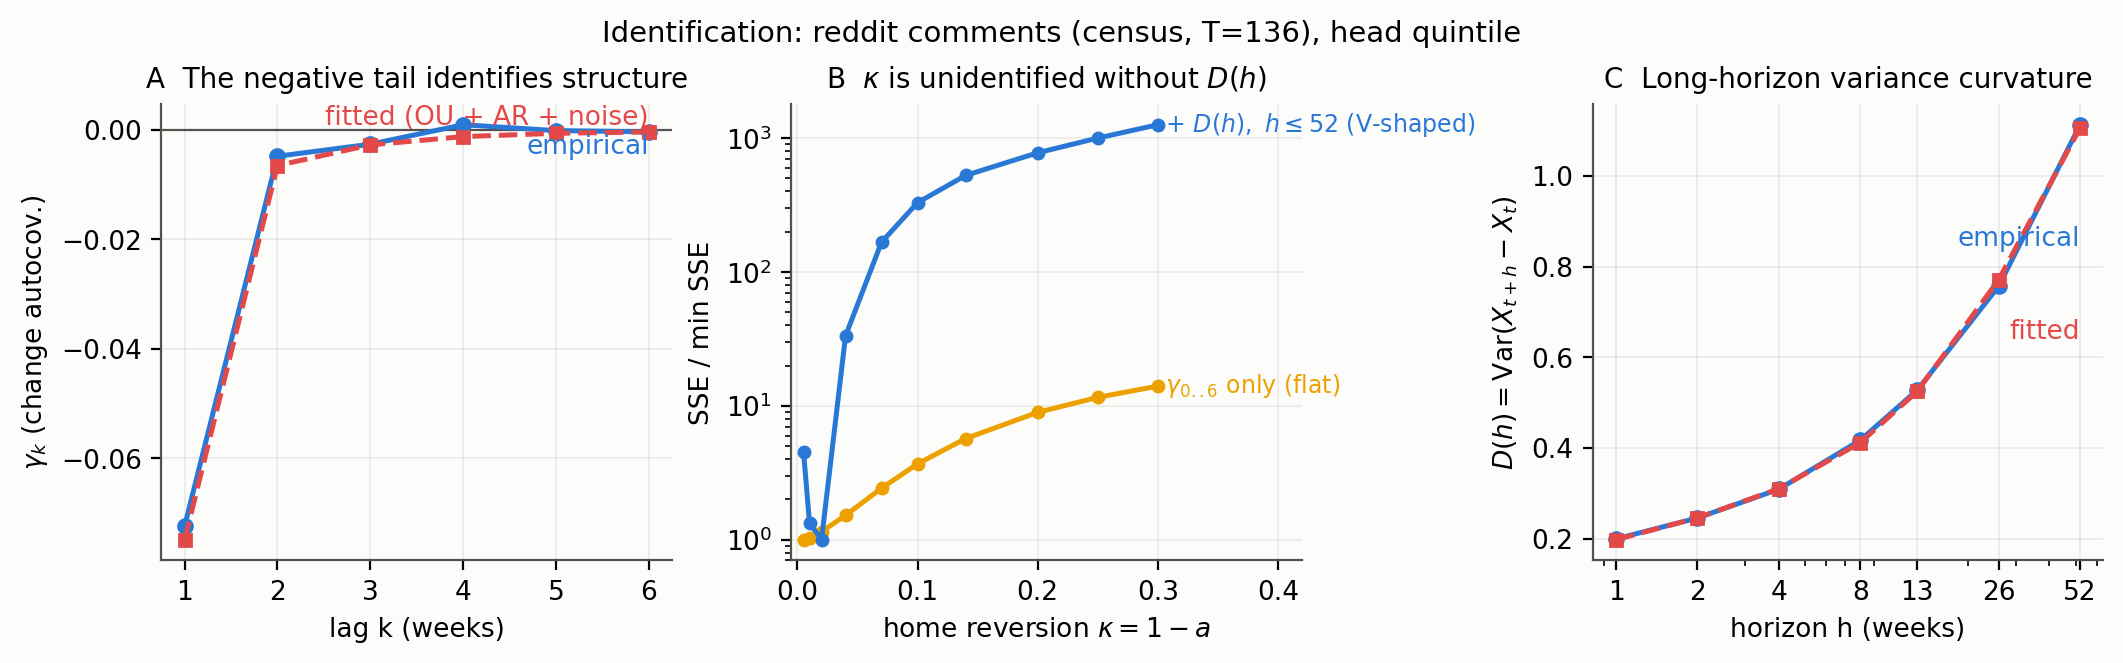
\includegraphics[width=0.94\textwidth]{fig2_identification}
\caption{\textbf{Fig.~2 spec — Identification, not just fit (EXISTS:
\texttt{figures/fig2\_identification.pdf}, built by
\texttt{llm\_fitting/make\_figures.py}).}
Reddit comments (census, T=136), head quintile.
(\emph{A}) Change-autocovariance tail $\gamma_{1..6}$, empirical vs fitted
(OU + AR + noise) — the negative tail is real structure, and the fit
captures it.
(\emph{B}) SSE profile over home-reversion $\kappa$: flat under
$\gamma_{0..6}$ alone, sharply V-shaped once $D(h)$, $h\le52$, joins the
moment vector — reader concludes $\kappa$ is IDENTIFIED by long-horizon
variances and unidentifiable without them (\S2i).
(\emph{C}) $D(h)$ curvature, empirical vs fitted through $h$ = 52 —
the identifying moments are themselves matched.
Reconciliation vs the E3 plan: matches; no changes needed.}
\label{fig:identification}
\end{figure*}

\begin{figure*}[p]
\centering
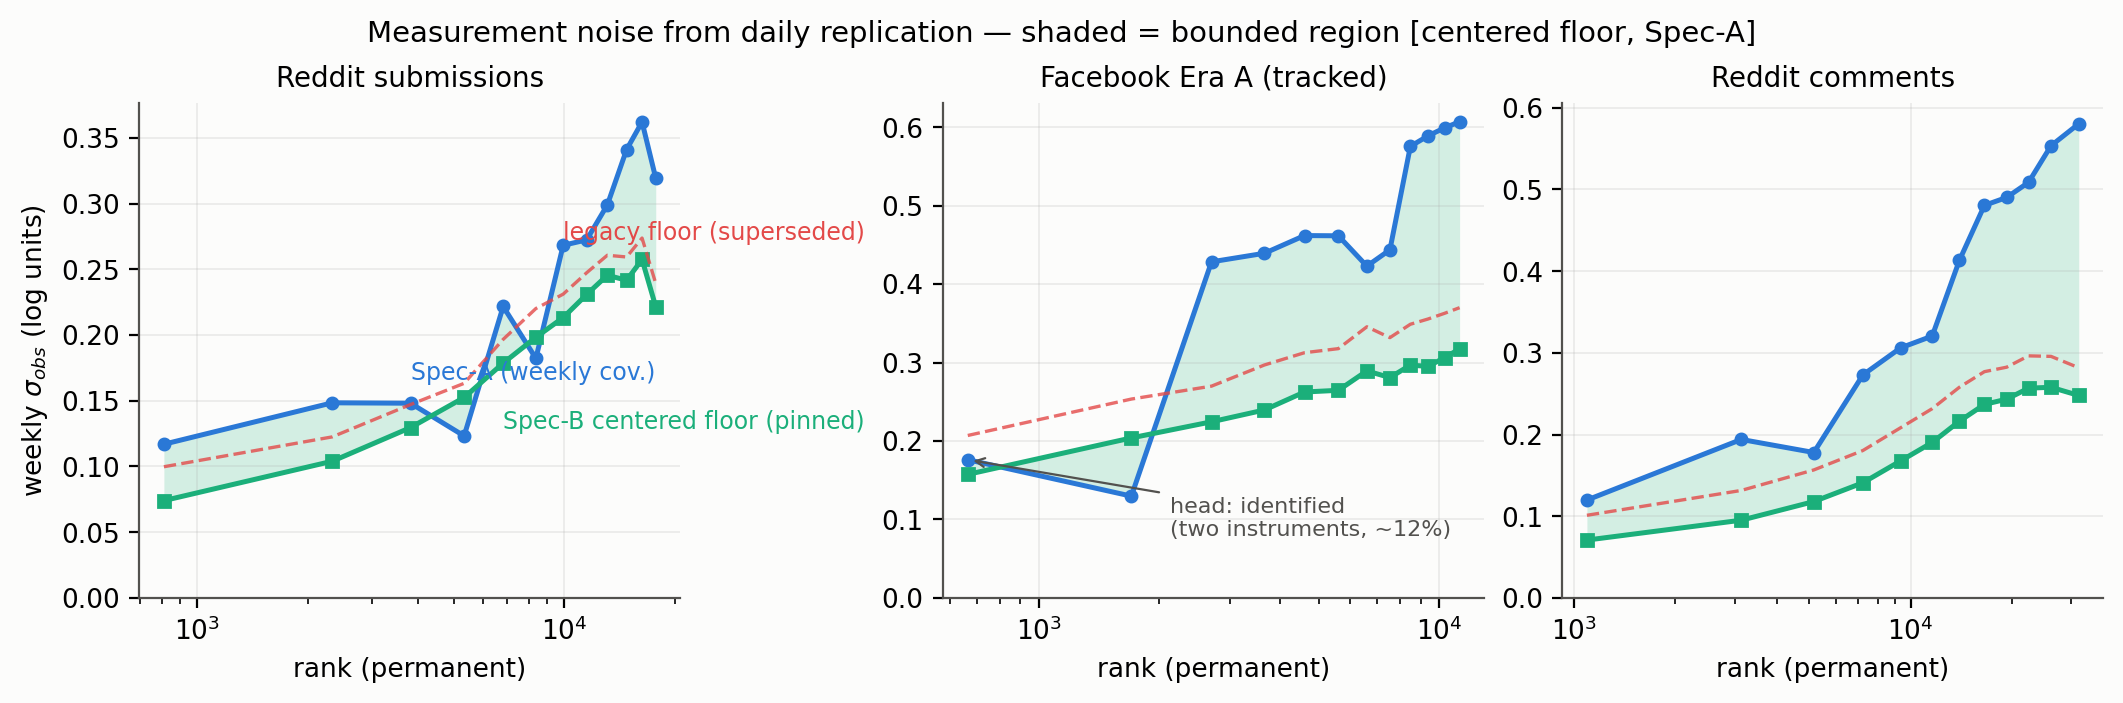
\includegraphics[width=0.94\textwidth]{fig3_sigma_obs}
\caption{\textbf{Fig.~3 spec — Measurement noise from daily replication
(EXISTS: \texttt{figures/fig3\_sigma\_obs.pdf}).}
Weekly $\sigma_{\mathrm{obs}}$ vs permanent rank, three panels (subs, FB
Era A tracked, comments): Spec-A weekly-covariance curve (upper), pinned
centered Spec-B floor (lower), superseded legacy floor as dashed reference;
shaded region = the bounded interval [centered floor, Spec-A]. FB head
annotated as IDENTIFIED (two instruments agree within $\sim$12\%, \S2r) —
reader concludes the noise level is measured, not assumed: identified in
shape everywhere, in level at the FB head, bracketed elsewhere, with the
bracket WIDENING with rank depth (the intermittency question, \S2h).
Reconciliation vs the E3 plan: "before/after pin" replaced by the dashed
legacy reference — keep as built.}
\label{fig:sigmaobs}
\end{figure*}

\begin{figure*}[p]
\centering
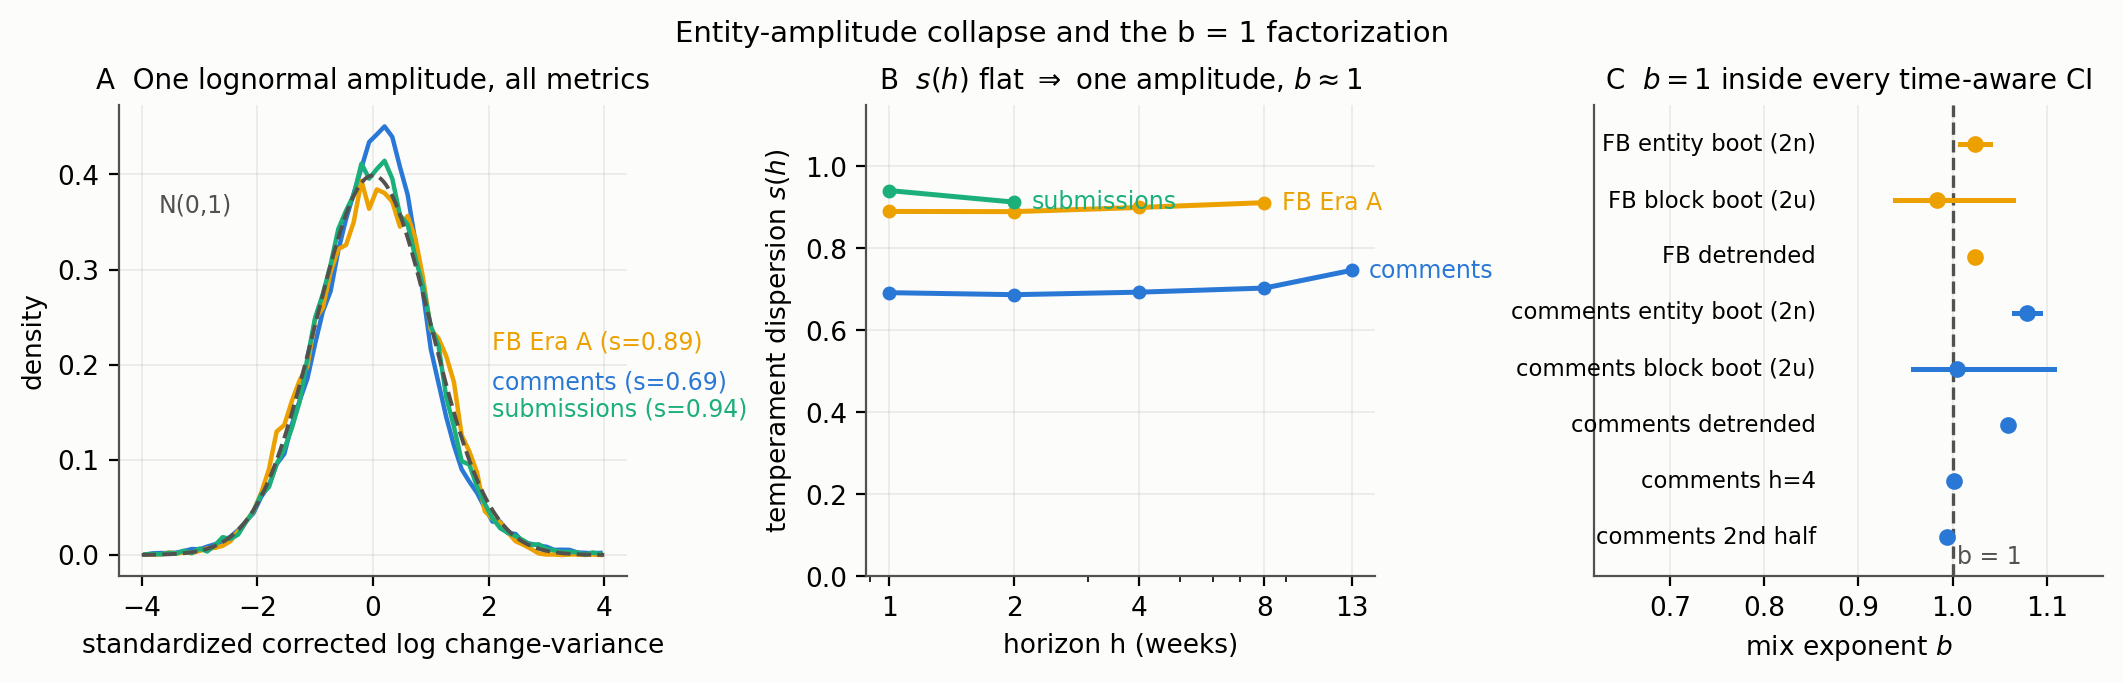
\includegraphics[width=0.94\textwidth]{fig4_amplitude}
\caption{\textbf{Fig.~4 spec — Entity-amplitude collapse and the $b=1$
factorization (EXISTS: \texttt{figures/fig4\_amplitude.pdf}).}
(\emph{A}) Standardized bias-corrected log change-variance densities for
all three metrics vs N(0,1) — one lognormal amplitude family across
metrics (spreads $s$ = 0.89 / 0.94 / 0.69, \S2h).
(\emph{B}) Temperament dispersion $s(h)$ vs horizon — FLAT, the instrument
behind $b\approx1$ (\S2l).
(\emph{C}) Forest plot of $b$ under every robustness variant (entity vs
block bootstrap, detrended, common-horizon, split-window) against the
$b=1$ line — reader concludes exact $b=1$ sits inside every time-aware CI
(\S2u).
Reconciliation vs the E3 plan: matches (E3's "corrected log-variance
distribution vs lognormal" = panel A).}
\label{fig:amplitude}
\end{figure*}

\begin{figure*}[p]
\centering
\fbox{\parbox[c][8cm][c]{0.94\textwidth}{\centering\sffamily
FIG 5 — DOES NOT EXIST YET.\\
Spec below; inputs are the recorded OOS gate outputs
(\texttt{rankdiff\_kalman.py --oos} runs per \S2s).}}
\caption{\textbf{Fig.~5 spec — Out-of-sample movement against persistence.}
(\emph{A}) Held-out rank-displacement distributions at $h$ = 1, 4, 13 for a
representative late split per panel: empirical vs model vs persistence
baseline — reader sees the model matches the DISTRIBUTION (median AND p90),
not just a summary (e.g. comments last split dRank1/4/13 = 6/8/11 vs emp
6/8/11, \S2l).
(\emph{B}) Per-split relative-error trajectories, model vs persistence, all
three panels (FB identified spec 0.118 $\pm$ 0.038 vs 0.145 $\pm$ 0.031
beating 4/5, \S2r; subs conditional 0.118 vs 0.168 beating 4/5, \S2f;
comments 0.159 vs 0.160 at par, \S2l) — splits shown individually because
they are dependent (\S2q C5), never as an averaged bar alone.
(\emph{C}) Coverage and Wasserstein summary per panel/spec, with the FB
calibrated Spec-A reference (0.114, 5/5) shown as the declared sensitivity
spec — the identified spec leads (\S2x binding ordering).
Caption must state: all estimation train-only; scale = 1.0 on 5/5 FB
identified splits (zero calibration freedom).}
\label{fig:oos}
\end{figure*}

%% ---- TABLE 1: the two-estimand stack matrix (verdict A4 made a display) -----
%% DISPLAY-ITEM DECISION: Table 1 = the stack/target matrix (the anti-
%% forking-paths display; must be main text). A Kawakatsu-2021-style
%% per-platform PARAMETER table (s, b vs the b=1 threshold, kappa range,
%% sigma_obs head bracket, rho_L, t-df — all from \S2h/\S2r/\S2u) is the
%% candidate SECOND table: main text only if the page budget allows a 7th
%% display item; otherwise SI Appendix Table S1, cited from R2 par. 1.
\begin{table*}[p]
\centering
\caption{\textbf{Table 1 spec — Specification $\times$ evaluation matrix
with explicit targets (from \S2s; the anti-forking-paths display).}
Rows = (panel $\times$ stack); columns = TARGET (structural reproduction /
OOS movement), in-sample card, churn error, OOS rel.\ err vs persistence,
CI coverage, calibration freedom used. Every cell filled INCLUDING the
failures (FB full stack OOS 0.170 vs 0.145, cov 20\% — loses, \S2s;
spec-B in-sample cards below structure stacks, \S2r). Footnote states the
scope condition mechanism (R3 par.\ 1) and that "15/15" is descriptive
(\S2x).}
\begin{tabular}{llllll}
Target & Panel & Stack & In-sample & OOS vs persistence & Coverage \\
\hline
\todo{fill from \S2s matrix} & & & & & \\
\end{tabular}
\label{tab:stacks}
\end{table*}

%% ============================================================================
%% ============================================================================
%%   SUPPORTING INFORMATION PLAN (outline only — becomes a separate SI
%%   Appendix PDF at submission; rendered here so the skeleton is complete)
%% ============================================================================
%% ============================================================================
\newpage
\section*{Supporting Information plan (outline; separate PDF at submission)}
{\footnotesize\sffamily

\textbf{SI-1 Instrument forensics and eras.} CrowdTangle era table
(A/B/C/M/D) with health series (pages/day, pages/week, enrollment); era
handling directives; low-count-day guard; Era C/D replication (transportable
quantities reproduce: s within 0.05, floor shape at +15--20\%, \S2g-X P4);
Era M mixture diagnosis (\S2g-X). Reddit census verification (0/943 flagged
days). Sources: \S2g, \S2g P0, instrument\_eras.py.

\textbf{SI-2 Universe and membership.} Coverage-K registration from
concentration alone; absence-penalized membership + the ghost-spiker
pitfall it fixes (with the locked test); buffer invariance; boundary-flux
anatomy (droppers land shallow, 99.93\% remain observed); membership-window
drift measured vs headline invariance (\S2b, \S2g-X P5, research\_notes
\S3).

\textbf{SI-3 Covariance derivations and identifiability.} Change-
autocovariance and D(h) formulas (review D1); mixture-of-exponentials /
Prony identifiability and the flat-SSE degeneracy theory (review D2/B3);
MD estimator consistency conditions and weighting robustness (identity vs
precision — inert, \S2y); temperament correction chain (review D4);
b-statistic exactness under the null and leading bias (review D5).

\textbf{SI-4 Spec-B derivation and the projection audit.} Delta-method map
from daily shares to the weekly floor; the CJC = 0 null direction; centered
vs legacy floor on all three platforms (head shifts $-24$ to $-30\%$); the
FB floor violation the legacy convention manufactured; re-pin reruns table
(every spec-B-dependent result, legacy vs centered) (\S2q, \S2r; review
B12/D7; test\_spec\_b\_projection.py).

\textbf{SI-5 Scorecard definitions, bands, and Q blocks.} The 15 moments
and thresholds; joint entity bootstrap + block bootstrap + MC band
construction; omnibus Q with shrinkage; per-block Q/df tables for all three
panels (\S2t, \S2y); Pers rows declared band-less/harsh; churn-row MC noise
(coll1 seed SD $\pm$0.15 at the head, \S2o).

\textbf{SI-6 OOS gate by split.} Per-split tables for every paper spec
(model vs persistence, scale, coverage, Wasserstein, held-out
distributions); split dependence caveat; MOM\_FLOOR rule and the one
degenerate split it retires (\S2f, \S2g-X P1, \S2l, \S2r; review C4/C5).

\textbf{SI-7 Rejected alternatives and the discovery chronology.} Import
SI\_DISCOVERY\_CHRONOLOGY.md verbatim (dated table: 16 discoveries/fixes,
6 negative results/retractions, 3 scope conditions, 2 external reviews);
rejected-alternatives register: fine-bands vs temperament battery (\S2c),
common volatility factor (\S2d), lifecycle-drift/scoring-filter/
survivor-composition kills (\S2p), missingness kill (\S2w), coll1
b-sensitivity retraction (\S2o), md-vr short-window scope (\S2i).

\textbf{SI-8 Confirmation protocol and results.} CONFIRMATION\_PROTOCOL.md
verbatim (frozen code commit, registered universe rule, E1--E4, pass
criteria, amendment A1 dated pre-data); results slots: E1 transport table
\todo{run}, E2 frozen gate \todo{run}, E3 card + Q vs surrogate-adjusted
target \todo{run}, E4 $\kappa_i$ concentration \todo{run}; discovery-vs-
confirmation panel map.

\textbf{SI-9 Negative-control and breadth panels.} Instagram as
measurement negative control (query-censored collection; why it is never
calibrated to, \S4); breadth systems as they land (Wikipedia pageviews
first): per-system s, b, s(h) flatness, OOS-vs-persistence, boundary flux
— the registered breadth claim set (\S2x item 2).

\textbf{SI-10 Data and code.} Pipeline description; frozen commit; data
availability and terms per source; reproduction commands (README block).
}

%% ============================================================================
%% BIBLIOGRAPHY PLAN (commented plan; keys ready for pnas-new.bst / a .bib
%% file to be created at drafting time). Organized by school; "cite for X".
%% Positioning note: the paper's differentiators vs the broader-but-shallower
%% ranking-dynamics school are (a) measurement-model identification, (b)
%% frozen out-of-sample validation, (c) instrument forensics — the citations
%% below are chosen so each differentiator has its methodological lineage
%% visible (UC econometrics for (a), forecasting-evaluation practice for (b),
%% era/instrument discipline for (c)).
%% ----------------------------------------------------------------------------
%% ATLAS MODELS / STOCHASTIC PORTFOLIO THEORY
%%   banner2005atlas      — Banner, Fernholz & Karatzas 2005, Ann. Appl.
%%                          Probab. — cite for rank-based diffusions; our
%%                          kappa as finite-N Atlas drift.
%%   ichiba2011hybrid     — Ichiba et al. 2011 — cite for hybrid
%%                          (multi-scale) Atlas drift, the two-timescale
%%                          home's lineage.
%% RANDOM GROWTH WITH BARRIER / SIZE DISTRIBUTIONS
%%   gabaix1999zipf       — Gabaix 1999 QJE — cite for Gibrat + reflecting
%%                          barrier -> Zipf; the rebirth mechanism.
%%   luttmer2007selection — Luttmer 2007 QJE — cite for entry/exit models
%%                          calibrated on upper-tail moments only.
%%   axtell2001zipf       — Axtell 2001 Science — cite for Zipf in firm
%%                          sizes; PNAS-audience touchstone.
%%   gabaix2016power      — Gabaix 2016 JEP — cite for the power-law survey
%%                          frame.
%%   gabaix2011rank       — Gabaix & Ibragimov 2011 — cite for rank-1/2
%%                          tail estimation (methods).
%%   clauset2009powerlaw  — Clauset, Shalizi & Newman 2009 — cite for tail
%%                          fitting discipline (methods).
%% RANKING-DYNAMICS UNIVERSALITY (the school this paper extends and
%% out-identifies)
%%   iniguez2022ranking   — I\~niguez, Pineda, Gershenson & Barab\'asi 2022,
%%                          Nat. Comms — cite for the ~30-system churn
%%                          regularities; contrast: no measurement model, no
%%                          OOS prediction.
%%   blumm2012ranking     — Blumm et al. 2012 PRL — cite for ranking-process
%%                          stability/fluctuation phases.
%% THE Q-MODEL (entity-amplitude precedent)
%%   sinatra2016quantifying — Sinatra et al. 2016 Science — cite for one
%%                          person-specific multiplier on a shared random-
%%                          impact rule; the b=1 factorization's named
%%                          analogue.
%% UNOBSERVED-COMPONENTS / PERMANENT-TRANSITORY ECONOMETRICS
%%   abowdcard1989        — Abowd & Card 1989 Econometrica — cite for
%%                          covariance-structure (MD) estimation of earnings
%%                          dynamics; our estimator's direct ancestor.
%%   hospido2012          — Hospido 2012 — cite for per-entity volatility
%%                          heterogeneity in earnings (temperament
%%                          precedent; slowly-drifting v_i).
%%   cochrane1988         — Cochrane 1988 JPE — cite for variance ratios /
%%                          long-difference identification of permanent
%%                          components.
%%   poterba1988          — Poterba & Summers 1988 JFE — cite for long-
%%                          horizon mean-reversion power (why D(h) moments).
%%   famafrench1988       — Fama & French 1988 JPE — companion cite to
%%                          poterba1988.
%%   stockwatson1998      — Stock & Watson 1998 JASA — cite for pile-up /
%%                          median-unbiased variance estimation (why the
%%                          noise split needs an instrument).
%%   harvey1989           — Harvey 1989 (book) — cite for structural time
%%                          series / fixing measurement noise externally.
%%   kamber2018           — Kamber, Morley & Wong 2018 REStat — cite for
%%                          constraining signal-to-noise when unconstrained
%%                          MLE is implausible.
%% SHRINKAGE
%%   smyth2004            — Smyth 2004 SAGMB (limma) — cite for the
%%                          digamma/trigamma log-variance moment machinery
%%                          behind s and EB v-hat.
%% ATTENTION DYNAMICS
%%   wu2007novelty        — Wu & Huberman 2007 PNAS — cite for collective-
%%                          attention decay (PNAS lineage).
%%   lorenzspreen2019     — Lorenz-Spreen et al. 2019 Nat. Comms — cite for
%%                          accelerating attention dynamics (contrast: item-
%%                          level bursts vs endpoint-level stationarity).
%%   hindman2018trap      — OPTIONAL: Hindman 2018, The Internet Trap —
%%                          cite for audience-concentration stakes in the
%%                          Discussion (author-adjacent; owner's call).
%% DATA / INSTRUMENTS
%%   baumgartner2020pushshift — Baumgartner et al. 2020 ICWSM — cite for the
%%                          Pushshift census.
%%   crowdtangle          — CrowdTangle Team, Meta — cite for the FB
%%                          instrument (tracked-panel caveats in SI-1).
%% ----------------------------------------------------------------------------
%% At drafting time: create pnas_outline.bib from these keys, switch to
%%   \bibliography{pnas_outline} with the shipped pnas-new.bst.
%% ============================================================================

%% \bibliography{pnas_outline}   % enable once the .bib exists

\end{document}
